\chapter{The Minkowski world}

\newpage
\thispagestyle{empty}
\begin{figure}[H]
\centering
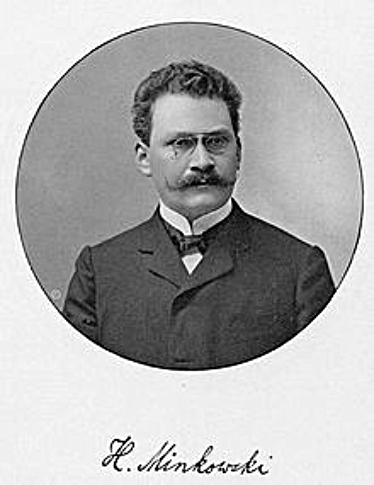
\includegraphics[scale=.5]{src/images/lbk-graphics/portraits/minkowski-wiki.jpg}
\caption*{Hermann Minkowski}
\end{figure}
%~ \portrait{.58}{lbk-graphics/portraits/minkowski-wiki.jpg}
%~ {Hermann Minkowski}
\begin{quote}
Hermann Minkowski (22 June 1864 - 12 January 1909) was a 
German mathematician and professor. He show\-ed in 1907 that 
the special theory of relativity of 1905, developed by his 
former student Albert Einstein, could be understood 
geometrically as a theory of four-dimen\-sional space-time, 
now known as the "Minkowski spacetime". Minkowski is also 
recognized for his contribution to the geometrical theory of 
numbers.
\hfill --Wikiquote
\newpage

From henceforth, space by itself, and time by itself, have 
vanished into the mere shadows and only a kind of blend of 
the two exists in its own right.\\\dm\hfill--Hermann 
Minkowski.\\---As quoted in J R Newman, J. R. Newman (ed.) 
\textsl{The World of Mathematics, New York: Simon and 
Schuster, 1956. Contributed by: Zaady}
\dm \vspace*{1\bsk}

The mathematical education of the young physicist (Albert 
Einstein) was not very solid, which I am in a good position 
to evaluate since he obtained it from me in Zurich some time 
ago \\ \dm \hfill-- Hermann Minkowski

\url{http://www-history.mcs.st-andrews.ac.uk
 /Quotations/Minkowski.html}
\end{quote}

%~ \newpage
%~ \vspace*{3\bsk}
\begin{quote}
\textsl{One of the greatest intellectual achievements of the 
twentieth century is surely the realisation that  space and 
time should be considered as a single whole--a four- 
dimensional manifold called  spacetime--rather than two 
separate, independent entities. This  resolved at one stroke 
the apparent incompatibility between equivalence of Lorentz  
observers and the constancy of the speed of light}

{\flushleft --{Malcolm Ludvigsen, {General Relativity: a 
geometric approach}, C.U.P., 1999, Cambridge, p.3.}}
\end{quote}

\newpage
\section{Introduction}

The Minkowski spacetime $\mbb{M}$, also called the 
\textbf{Minkowski world}, is a real four-dimensional 
manifold endowed with an {indefinite metric}.  Points 
of  $\mbb{M}$ are also called \textbf{events}. 
$\,\mbb{M}$ admits an infinite class of (real)  global 
coordinate systems called  \textsl{pseudo-Cartesian 
systems}, each one of which covers the \textsl{whole 
of} $\mbb{M}$. 
A \textbf{pseudo-Cartesian coordinate system} in 
$\mbb{M}$, say, $S\equiv \{x^\gkm\}, \gkm=0,1,2,3$, is 
a real four-dimensional coordinate system in which all 
the four coordinates  $x^0, x^1, x^3, x^3$ range over 
the domains $-\infty < x^0, x^1$, $x^3, x^3< \infty$. As 
already said, in any such pseudo-Cartesian coordinate 
system, there is a one-to-one correspondence between 
events of $\mbb{M}$ and coordinate quadruplets $(x^0, 
x^1,x^2x^3)$ throughout $\mbb{M}$. One says $\mbb{M}$ 
is a global  coordinate systemwhich covers the 
\textsl{whole of} $\mbb{M}$.  In physics, any such    
pseudo-Cartesian coordinate system $\{x^\gkm\}$ is said 
to provide a \textbf{Lorentz frame}. In his book, we 
also use these phrases ``Lorentz frame'' and ``Lorentz 
coordinate system'' interchangeably.

\index{Minkowski world ! events}
 
To simplify notation, we often denote the time and space 
coordinates  in a pseudo-Cartesian system $S:\{x^\gkm\}$  
by $(w\equiv x^0 \equiv ct, x^1 \equiv x, x^2 \equiv  y, 
x^3 \equiv z)$.   
                                                  
To facilitate the use of \textbf{matrix methods}, we 
associate with an event $P$ marked by coordinates 
$(w,x,y,z)$ and $(w',x',y',z')$ in the Lorentz frames $S$ 
and $S'$ respectively,  the \textsl{column matrices}
\begin{align*}
X=\begin{pmatrix} w\\x\\y\\z\end{pmatrix} ,\;
X'=\begin{pmatrix} w'\\x'\\y'\\z'\end{pmatrix} ,
\end{align*}
and the corresponding \textsl{row matrices}\footnote{An 
overhead ``tilde'' denotes matrix transposition.}
\begin{align*}
\tilde{X}=\begin{pmatrix}
 w& x& y& z 
\end{pmatrix} ,\;
\tilde{X}'=\begin{pmatrix}
w'&x'&y'&z' 
\end{pmatrix}.
\end{align*}
\subsection{Review of Lorentz transformations} 
A \textsl{homogeneous Lorentz transformation} (cf. 
\S~13.7)  relating the time and space coordinates of an 
event $P$ in the two Lorentz frames $S':\{x^\gkmp\}$ 
and $S:\{x^\gkm\}$ may be expressed in matrix notation 
as
\begin{align}\label{mw.1}
X'=LX= \begin{pmatrix}
x^{0'}\\x^{1'}\\x^{2'}\\x^{3'}\end{pmatrix}
=\begin{pmatrix}
 ?L^{0'}_0?&  ?L^{0'}_1?&  ?L^{0'}_2? &?L^{0'}_3?\\
 ?L^{1'}_0?&  ?L^{1'}_1?&  ?L^{1'}_2? &?L^{1'}_3?\\
 ?L^{2'}_0?&  ?L^{2'}_1?&  ?L^{2'}_2? &?L^{2'}_3?\\
 ?L^{3}_0? &  ?L^{3}_1? &  ?L^{3}_2?  &?L^{3}_3?\\
\end{pmatrix}
\begin{pmatrix}
x^{0}\\x^{1}\\x^{2}\\x^{3}
\end{pmatrix} ,
\end{align}
Here, in \eqref{mw.1}, $X'$ and $X$ are the column 
matrices representing the event $P$ respectively in the 
Lorentz frames $S'$ and $S$. The elements of  $X'$ and 
$X$ are the time-space coordinates of  the event $P$ in 
the Lorentz frames $S'$ and $S$. The real $4\times 4$ 
matrix $L\equiv (\mtud{L}{\gkmp}{\gkn}), 
\;\gkmp,\gkn=0,1,2,3,$ in \eqref{mw.1} is called a 
\textsl{Lorentz matrix}.  The Lorentz matrix $L$, by 
its definition, satisfies the \textsl{Lorentz 
condition}
\begin{align}\label{mw.2}
\boxed{\tilde{L}\gky L =\gky},
\end{align}
where $\tilde{L}$ is the matrix transpose of $L$
and 
\begin{align}\label{mw.3}
\gky=(\gky_{\gkm\gkn})=
\begin{pmatrix}
1&0&0&0\\0&-1&0&0\\0&0&-1&0\\0&0&0&-1
\end{pmatrix} ,
\end{align}
is a $4\times 4$ constant  matrix called the 
\textsl{Minkowski metric}. In terms 
of matrix elements, the Lorentz condition \ie, Eqn. 
\eqref{mw.2}, may be written as
\begin{align}\label{mw.4}
\boxed{\gky_{\gkmp\gknp}\,\mtud{L}{\gkmp}{\gka}
\,\mtud{L}{\gknp}{\gkb} 
=\gky_{\gka\gkb}},
\end{align}
where, as is usual, in any matrix element, the 
left-suffix is  the row-index and the right-suffix is  
the column-index (For instance, 
$\mtud{L}{\gkmp}{\gka}$ is the element in the 
$\gka$-th row of the matrix $L$.) Also, we may note 
that we have used the \textbf{summation convention} of 
summing over  repeated indices from $0$ to $3$ in 
equation \eqref{mw.4}. \subsection{The inverse Lorentz 
matrix} \hbf{Notation} In this chapter, we use the 
symbol ${\what{A}}$ to denote the inverse $A^{-1}$ of 
a (non-singular) matrix $A$. This notation is 
convenient while referring to the elements of the 
inverse matrix $A^{-1}$: for instance, we may 
denote $?{(A^{-1})}^{\gka}_{\gkb}?$ 
compactly as $?{\what{A}}^{\gka}_{\gkb}?$.

\hbf{The inverse Lorentz matrix} Observe that if 
multiply Eqn.\eqref{mw.2} by $\gky$, and use the 
relation $\gky^2=E$, we get $\gky \tilde{L} \gky L=E$  
where $E$ is the $4\times 4$ unit matrix. Further, if 
we right-multiply this equation by $ L^{-1}$, we get 
${\what{L}}\equiv L^{-1} =\gky \tilde{L} \gky$ for the 
inverse Lorentz matrix. Using this expression $\gky 
\tilde{L} \gky$ for ${\what{L}}$, we may express the 
elements of ${\what{L}}$ in terms of  the elements of  
${\what{L}}$ as follows:\vspace{.5\bsk}
\begin{align}\label{mw.5}
&\hspace*{-9mm}\what{L}\nnt= \nnt\begin{pmatrix}
?{\what{L}}^{0}_{0}? &?{\what{L}}^{0}_{1}?&
?{\what{L}}^{0}_{2}? &?{\what{L}}^{0}_{3}?\\
?{\what{L}}^{1}_{0}? &?{\what{L}}^{1}_{1}?&
?{\what{L}}^{1}_{2}? &?{\what{L}}^{1}_{3}?\\
?{\what{L}}^{2}_{0}? &?{\what{L}}^{2}_{1}?&
?{\what{L}}^{2}_{2}? &?{\what{L}}^{2}_{3}?\\
?{\what{L}}^{3}_{0}? &?{\what{L}}^{3}_{1}?&
?{\what{L}}^{3}_{2}? &?{\what{L}}^{3}_{3}?\\
\end{pmatrix} \nnt= \nnt
\begin{pmatrix}
 ?L^{0}_0?& -?L^{0}_1?& -?L^{0}_2? & -?L^{0}_3?\\
-?L^{1}_0?&  ?L^{1}_1?&  ?L^{1}_2? &  ?L^{1'}_3?\\
-?L^{2}_0?&  ?L^{2}_1?&  ?L^{2}_2? & ?L^{2}_3?\\
-?L^{3'}_0?&  ?L^{3'}_1?&  ?L^{3'}_2? & ?L^{3'}_3?\\
\end{pmatrix}\,.
\end{align}

\section{4-tensors}
Minkowski tensors, also called 4-tensors, are a part of 
the geometrical structure on the Minkowski manifold 
$\mathbb{M}$ and they are essential for a study of the 
special theory of relativity.

\hbf{Notation} We denote 4-scalars (\ie, 4-tensors of 
rank zero) by  lowercase Greek characters such as 
$\varphi, \psi, \dt$. We denote all other higher rank 
4-tensors by bold-face upper-case 'mathbf' 
characters\footnote{While writing by the hand, one may 
denote 4-tensors by an upper case character with an 
underline as in $\underline{A}$, $\underline{B}\dt$, or 
by the familiar wriggly underline.} such as 
$\mathbf{A}, \mathbf{B}, \mathbf{C}$. This notation 
does not display the ranks of the 4-tensors; however, 
we may verbally mention the rank of the tensor if need 
be. 

Along with the above described \textsl{coordinate-free 
notation} for tensors, which we use occasionally,  we 
generally use the \textbf{compo\-nent-notation} for 
tensors. This notation provides an access to a tensor 
through its components relative to a coordinate basis.
Lower-case Greek characters such as $\gkl, \gkm, \gkn \dt$, 
as usual,  are used for sub-scripts and super-scripts on 
tensor-components. As an example, we  may note that the 
contravariant components of a 4-vector $\mathbf{A}$ are 
denoted by $A^{\gkmp}$ and $A^{\gkm}$ in the primed and 
un-primed Lorentz coordinate systems. Similarly, 
$?F^{\gkmp}_{\nnt\gknp}?$\,, $F_{\gkmp\gknp}$, 
$?F^{\gkm}_{\gkn}?$, $F_{\gkm\gkn}$, etc.,  denote the 
various mixed, contra and co-variant components of a second 
rank 4-tensor $\mathbf{F}$.

The reader may also find plenty of phrases such as 
``\textsl{$A^{\gkm}$ is a 4-contravector}'', 
``\textsl{$A_{\gkm\gkn}$ is a second rank covariant 
4-tensor}'' and so on, in this book (also). Having picked 
up these phrases as students in the physics class, we 
continue with them as a matter of (convenient) habit. In 
fact, these phrases must only be understood as abbreviations 
for the more correct longer phrases such as ``$A^{\gkm}$ are 
the contravariant components of the 4-vector $\mathbf{A}$ in 
 the Lorentz coordinate system $S$\;'', ``$A_{\gkm\gkn}$ 
are the covariant components of the second rank 4-tensor 
$\mathbf{A}$'', and so on.

Also, in what follows, we shall be repeatedly referring to 
the 'forward' and 'inverse'  Lorentz 
transformations connecting  two arbitrary Lorentz 
frames $S:\{x^\gkm\}$ and $S':\{x^{\gkmp}\}$: They are 
given by
\begin{align}\label{mw.6}
&\text{The \textit{forward} Lorentz 
transformation:}\quad 
x^{\gkmp} 
=\mtud{L}{\gkmp}{\gkn}\,x^\gkn,\\
&\text{The \textit{inverse} Lorentz 
transformation:}\;\;\quad 
x^{\gkm} =\mtud{\what{L}}{\gkm}{\gknp}\,x^\gknp. 
\label{mw.7}
\end{align} 


\subsection{4-scalars}\index{4-scalar}
\dfnb  A mathematical object $\mathbf{\varphi}$ which 
is specified by the \textbf{same, single,  real number} 
in all Lorentz frames is called a \textbf{4-scalar}. 
Under the homogeneous Lorentz transformations 
\eqref{mw.6} and \eqref{mw.7} a 4-scalar remains 
unchanged:
\begin{align}\label{mw.8}\mathbb{}
\varphi'=\varphi.
\end{align}
One also says that \eqref{mw.8} is the ``transformation 
rule'' of a 4-scalar under Lorentz 
transformations\footnote{Throughout this book, we 
 deal with only homogeneous Lorentz transformations. 
As such the shorter phrase ''Lorentz transformation'', 
unless otherwise stated, refers to  homogeneous 
Lorentz transformations only.}.

\subsection{Contravariant components of a  
4-vector}\index{4-vector ! contravariant components} 
The  transformation rule of the contravariant 
components of a 4-vector under the Lorentz 
transformation \eqref{mw.6} is
\begin{align}\label{mw.9}
A^{\gkmp}= \frac{\dow x^{\gkmp}}
{\dow x^\gkn}A^\gkn= 
\mtud{L}{\gkmp}{\gkn}\,A^\gkn.
\end{align}

\newpage

Note that \eqref{mw.9} is precisely the transformation 
rule \eqref{mw.6} of the coordinates $x^\gkm$ of an 
event under a Lorentz transformation; in fact, 
\textsl{$x^\gkm$ is the prototype of a 
4-contravector}\footnote{On a general manifold, 
however, the coordinates $x^\gkm$ of a point do 
\textit{not} transform like the components of a 
contravector; then, only their differentials $dx^\gkm$ 
transform like the components of a contravector.}.

It is customary to say Eqn.\eqref{mw.9} is the 
``transformation law of a 4-contravector''. This statement  
should also be understood as a shorthand for ``the 
transformation law of the contravariant components of a 
4-vector''. It is important to note that a 4-vector 
$\mathbf{A}$ is an \textit{invariant object}, 
sometimes called a \textit{4-vector invariant}, and 
\textit{it does not change} under a Lorentz transformation. 
Only its components, contravariant, or, 
covariant, change under a Lorentz transformation. This 
remark also applies for 4-tensors of other higher ranks. As 
a last passing remark on the customary usage of the word 
tensor, we note that in Exercise~5.3 at the end of this 
chapter, we say that ``the Kronecker delta 
$?\delta^\gkm_\gkn? $ is a 4-tensor of the type $ (1,1) 
$''. Now it should be obvious that this really means that  
$?\delta^\gkm_\gkn?$ are the $(1,1)$-components of a 
4-tensor of  rank 2.

\subsection{Covariant components of a 
4-vector}\index{4-vector ! covariant components} Note 
that a 4-vector $\mathbf{A}$ may also be defined by 
specifying its (four, real) covariant components in any 
one Lorentz coordinate system, say $S:\{x^\gkm\}$, and 
\textit{obtaining} the components of $\mathbf{A}$ in 
all Lorentz frames $S':\{x^{\gkmp}\}$ by appealing to  
the transformation rule
\begin{align}\label{mw.10}
A_{\gkmp}=\frac{\dow x^\gkn}{\dow 
x^{\gkmp}}A_\gkn=?{\what{L}}^{\gkn}_{\gkmp}?A_\gkn.
\end{align}
This  is the \textsl{Lorentz transformation rule of the  
covariant components of a 4-vector}. \hbf{The gradient of a 
4-scalar}\index{4-scalar ! gradient of a} Using the familiar 
chain rule of partial derivatives, we note that the gradient 
$\dow_\gkm\varphi$ of a 4-scalar field transforms under the 
Lorentz transformation \eqref{mw.6} as
\begin{align}\label{mw.11}
\dow_{\gkmp}\varphi
=\frac{\dow \varphi}{\dow x'^\gkm}
=\frac{\dow x^\gkn}{\dow x^{\gkmp}}\frac{\dow 
\varphi}{\dow x^\gkn} 
=\mtud{\what{L}}{\gkn}{\gkmp}\,\dow_\gkn\varphi.
\end{align}
This is precisely Eqn.\eqref{mw.9} with $\dow_\gkn\varphi$ 
in the place of $A_\gkn$. Thus, \textsl{the gradient 
$\dow_\gkm\varphi $ of a 4-scalar field $\varphi$ 
is the prototype of a covariant 4-vector.}

\subsection{Jacobian identities}\index{Jacobian 
identities}

We may recall that the Lorentz matrix $L$ in 
\eqref{mw.1} and its inverse $\what{L}$ in \eqref{mw.5} 
are actually the Jacobian matrices of the forward and 
inverse Lorentz transformations \eqref{mw.5} and 
\eqref{mw.6}. This obsrvation leads to the following 
\textsl{Jacobian identities}:
\begin{align}\label{mw.12}
\mtud{\what{L}}{\gkm}{\gka'}\mtud{L }{\gka'}{\gkn}
=\boxed{\frac{\dow x^\gkm}{\dow x^{\gka'}}\,\frac{\dow 
x^{\gka'}}{\dow x^\gkn}=\frac{\dow x^\gkm}{\dow 
x^\gkn}=\mtud{\delta}{\gkm}{\gkn}}
\end{align}
and
\begin{align}\label{mw.13}
&\mtud{L}{\gkmp}{\gka}\mtud{\what{L}}{\gka}{\gknp}
=\boxed{\frac{\dow x^{\gkmp}}{\dow x^\gka}\,\frac{\dow 
x^\gka}{\dow x^{\gknp}}=\frac{ \dow x^{\gkmp}}{\dow 
x^{\gknp}}=\mtud{\delta}{\gkmp}{\gknp}}
\end{align}
These  (boxed) identities come in handy in  the 
manipulation of expressions involving  
tensor-components.

\subsection{4-tensors of higher rank}\index{4-tensor}

\hbf{Transformation law of the $(r,s)$-components of  
4-tensor of rank ($r+s$)} With every pair of numbers 
chosen from the set $r,\,s=0,1,2,3,\dots$, we may 
define a 4-tensor $\mathbf{A}$  of rank $(r+s)$ by 
specifying all its components $?A^{{\gkm_1}\dots 
{\gkm_r}}_{{\gkn_1}\dots {\gkn_s}}?$ in any one of the  
Lorentz coordinate systems, say, $S:\{x^\gkm\}$ and 
calculating  its components in other Lorentz 
coordinate system $S':\{x^\gkmp\}$ by appealing to the 
transformation law: 
\begin{align}\label{mw.14}
&?A^{{\gkmp_1}\dots {\gkmp_r}}_{{\gknp_1}\dots
{\gknp_s}}?\notag\\
&=\frac{\dow x^{\gkmp_1}} {\dow x^{\gka_1}} 
\dots\frac{\dow x^{\gkmp_r}}{\dow x^{\gka_r}} \,\,
\frac{\dow x^{\gkb_1}}{\dow x^{\gknp_1}}\dots
\frac{\dow x^{\gkb_s}} {\dow x^{\gknp_s}} 
?A^{{\gka_1}\dots
{\gka_r}}_{{\gkb_1}\dots {\gkb_s}}? \notag\\
&= ?L^{\gkmp_1}_{\gka_1}?\dots ?L^{\gkmp_r}_{\gka_r}?
\,\,\mtud{\what{L}}{\gkb_1}{\gknp_1} \dots
\mtud{\what{L}}{\gkb_s}{\gknp_s}\,\,?A^{{\gka_1}\dots 
{\gka_r}}_{{\gkb_1}\dots {\gkb_s}}?\;.
\end{align}
 \dfnb The number $r+s$ is called the \textbf{rank} of 
the tensor $\mathbf{A}$ defined by the transformation 
law in \eqref{mw.14} above. An $(r,s)$-component of a 
tensor $\mathbf{A}$ of rank ($r+s$) is labelled by $r$ 
superscripts and $s$ subscripts. 
\index{4-tensor ! rank of a}

\hbf{Free and dummy indices}\index{Free and dummy 
indices} A \textit{free index} is an index which occurs 
only once in a tensor expression. Unlike a free index, 
a \textit{dummy index} occurs precisely twice in a 
tensor expression, once as a superscript and once as a 
subscript, and indicates a summation from 0 to 3. The 
examples below should make the idea clear:
\begin{enumerate}
\item $?A^{\gka\gkb}{\gkg}?$ has three free indices 
$\gka,\gkb$ and $\gkg$. \item $?T^{\gka\gkb}_{\gkb}?$  
has one free index $\gka$ and one dummy index-pair  
$\gkb$.
\item The product $?A^{\gka\gkb}_{\gkg}? 
?T^{\gkg\gks}_{\gkb}?$        has two  free indices in 
$\gka$   and $\gks$, and two dummies $\gkb$ and $\gkg$. 
\item However, in the sum $(?A^{\gka\gkb}_{\gkg}? 
+?B{\gka\gkb}_{\gkg}?) $, although all the indices in 
$\gka\;\gkb$ and $\gkg$ occur twice in the sum, they do 
not have the 'signature' of dummies: (i)~They occur in 
different terms separated by the '\textbf{plus}' sign 
and (ii)~the repeated index pairs do not occur once as 
an upper index and once as a lower index. As such they 
are  \textbf{not dummies} and are free indices.
\end{enumerate}

In passing, we note that 4-vectors are regarded as  
4-tensors of the rank one and 4-scalars as 4-tensors of 
the rank zero. Hence, the name 4-tensors would apply to 
4-scalars, 4-vectors and all other 4-tensors of rank 
greater than one.

\section{Algebra of 4-tensors}\index{4-tensor ! 
algebra}

\hbf{The zero 4-tensors} \index{4-tensor ! 
zeros}

\defn A 4-tensor of rank $n$ \textbf{all} whose
components vanish in any one Lorentz coordinate 
system, is a \textbf{zero tensor of rank $n$}.

\hbf{Note}There is a zero tensor of every possible rank 
$n$ where $n=0,1,2,3,.. $.

As an example, consider a zero-4-tensor $\mathbf{A}$ 
of rank 2. Then, as per the above definition, every one 
of 
its components, namely,  $?A^\gkm\gkn?$, 
$?A^\gkm_\gkn?$, $?A_\gkm^\gkn?$,   and $?A_\gkm\gkn?$, 
vanishes in some Lorentz coordinate system, say,  
$S:\{x^\gkm\}$. 
Now, because the Lorentz transformation 
between any two Lorentz coordinate system is linear 
and homogeneous, every one of the components 
of this tensor $\mathbf{A}$ would vanish in every other 
Lorentz coordinate system $S':\{x^{\gkmp}\}$ obtained 
from $S:\{x^\gkm\}$ by a Lorentz transformation. 

\hbf{Scalar multiple of a 4-tensor} 
\index{4-tensor ! scalar multiple of a}
If $ \gkl $ is a 4-scalar and $\mathbf{A}$ is a  
4-tensor of rank $n$, then the scalar multiple of 
$\mathbf{A}$ by $\gkl$, denoted by $\gkl\mathbf{A}$, is 
a new 4-tensor of the same rank $n$. In a Lorentz 
coordinate system $S:\{x^{\gkm}\}$, the tensor 
$\gkl\mathbf{A}$ has the 
$(r,s)$-components\footnote{$s=n-r,\;r=0,1,2,\dt, n$} 
$\gkl ?A^{{\gka_1}\dots {\gka_r}}_{{\gkb_1}\dots 
{\gkb_s}}?$.

\hbf{Linear combination of 4-tensors}\index{4-tensor ! 
linear combination} If $\mathbf{A}$ and $ \mathbf{B}$ 
are two  4-tensors of the \textbf{same} rank, say 
$(r+s)$, and if $\gkl$ and $\gkm$ are two 4-scalars, 
then a new 
tensor  $\mathbf{C}\equiv \gkl\mathbf{A} + \gkm 
\mathbf{B}$ called the  the linear 
combination of these two tensors, is defined 
as follows: If 
$?A^{{\gka_1}\dots {\gka_r}}_{{\gkb_1}\dots {\gkb_s}}?$ 
and $?B^{{\gka_1}\dots {\gka_r}}_{{\gkb_1}\dots 
{\gkb_s}}?$ are the $S$-frame\footnote{Recall that we 
call a Lorentz coordinate system shortly as a 'Lorentz 
frame'. Here, $S$-frame means  the Lorentz coordinate 
system $S: \{x^\gkm\}$.}  $(r,s)$-components of 
$\mathbf{A}$ and $\mathbf{B}$, in the $S$-frame
\begin{align*}
?C^{{\gka_1}\dots {\gka_r}}_{{\gkb_1}\dots 
{\gkb_s}}? \equiv
\gkl ?A^{{\gka_1}\dots {\gka_r}}_{{\gkb_1}\dots 
{\gkb_s}}? +
\gkm ?B^{{\gka_1}\dots {\gka_r}}_{{\gkb_1}\dots
{\gkb_s}}?,
\end{align*}
are the $S$-frame components of $\mathbf{C}$.

\hbf{Sum and difference of 4-tensors} 
\index{4-tensor ! sum and difference} 
In the linear combination $\mathbf{C}$, defined above,  
if we set   $\gkl=1=\gkm$, we get the \textbf{sum} 
tensor $\mathbf{A} + \mathbf{B}$ whose $S$-frame  
$(r,s)$-components are  $?A^{{\gka_1}\dots 
{\gka_r}}_{{\gkb_1}\dots {\gkb_s}}?  +  
?B^{{\gka_1}\dots {\gka_r}}_{{\gkb_1}
\dots {\gkb_s}}?$.

Similarly, setting  $\gkl=1=-\gkm$ in the linear 
combination $\mathbf{C}$ defined above, we get     the 
\textit{difference} 4-tensor $\mathbf{A} - \mathbf{B}$ 
with the $S$-frame $(r,s)$-components  
$?A^{{\gka_1}\dots {\gka_r}}_{{\gkb_1} \dots {\gkb_s}}? 
+  ?B^{{\gka_1}\dots {\gka_r}}_{{\gkb_1}\dots 
{\gkb_s}}?$. Another difference tensor $\mathbf{B} - 
\mathbf{A}$ may be similarly defined.

\hbf{Note} Linear combinations, sums and 
differences of tensors are defined only for tensors of 
the \textbf{same rank}. More importantly, to obtain 
the $(r,s)$ components of a
linearly-combined tensor, we must combine the $(r,s)$ 
components of the constituent tensors appropriately.

\hbf{Outer product of 4-tensors} \index{4-tensor ! 
outer product} 
If $\mathbf{A}$ and $\mathbf{B}$ are two 4-tensors of 
arbitrary rank, and have  $(r,s)$ and $(p,q)$ 
components in the $S$-frame given by $ 
?A^{{\gka_1}\dots {\gka_r}}_{{\gkb_1} \dots {\gkb_s}}? 
$ and $ ?B^{{\gkm_1}\dots {\gkm_p}}_{{\gkn_1}\dots 
{\gkn_q}}? \;$, then their \textit{outer product} 
denoted by $ \mathbf{A} \otimes \mathbf{B} $  is a 
4-tensor of the rank $ (r+p+s+q) $ and has, in the 
$S$-frame, components of the type $(r+p,s+q)$ given by  
$?A^{{\gka_1}\dots {\gka_r}}_{{\gkb_1}\dots 
{\gkb_s}}? ?B^{{\gkm_1}\dots 
{\gkm_p}}_{{\gkn_1}\dots {\gkn_q}}?$.

We may observe that the scalar multiple $ \gkl 
\mathbf{A} $ is also an outer product, namely, that of 
a 4-tensor $\mathbf{A}$,  say, of rank $n$,  with the 
4-tensor $\gkl$ of rank $0$ and it is again 4-tensor of 
the same rank $n+0=n$. 

The rank of the outer product is the sum of the ranks 
of the factor tensors. 

Also, in general, the two outer products 
$\mathbf{A}\otimes \mathbf{B}$ and  $\mathbf{B} \otimes 
\mathbf{A}$ are not equal:  To see this in 
a particular case, consider the two vectors 
\begin{align*}
\mathbf{A} 
=\begin{pmatrix}A^0\\A^1\\A^2\\A^3\end{pmatrix} 
=\begin{pmatrix}2\\3\\1\\0\end{pmatrix} \quad 
\text{and} 
\quad \mathbf{B}=
\begin{pmatrix}B^0\\B^1\\B^2\\B^3\end{pmatrix} 
=\begin{pmatrix}2\\3\\1\\4\end{pmatrix}.
\end{align*}
Let us  form their outer products  
$\mathbf{C}\equiv \mathbf{A} \otimes 
\mathbf{B}$ and $\mathbf{C'}\equiv \mathbf{B} 
\otimes \mathbf{A}$. Then, we have, in particular, 
\begin{align*}
\hspace*{-5mm}?C^{13}?=A^1 B^3=3\times4=12,      
\text{ and }  
?{C}^{'13}?=B^1 A^3=3\times0=0,  
\end{align*}
which clearly shows that $\mathbf{A} 
\otimes \mathbf{B}\neq\mathbf{B} 
\otimes \mathbf{A}$.

\subsection{Contraction}
\index{4-tensor ! contraction}
From a 4-tensor $\mathbf{A}$ of the type $ (r,s)$, with 
components\break $?A^{\gkl_1 \gkl_2 
\dots \gkl_r}_{\gkm_1 \gkm_2 \dots   \gkm_s}?$
we may form a 4-tensor of the type $(r-1,s-1)$ as 
follows: We select a pair of \textit{unlike indices} 
(i.e., one upper and one lower 
index), say,  $\gkl_1$ and $\gkm_1$, set  $\gkl_1 
=\gkm_1=\rho$ and sum over the resulting pair of dummy 
indices $\{\rho,\rho\}$. Then, we obtain a tensor of 
the type $(r-1,s-1)$
whose components are the sums 
$\sum_{\gkr=0}^{3}?A^{\gkr \gkl_2 \dots \gkl_r}_{\gkr 
\gkm_2 \dots \gkm_s}?$. This tensor  is    called 
\textbf{a contraction of} $\mathbf{A}$.

\exm Obtain the contractions of 
$\mathbf{A}:?A^{\gka\gkb}_\gks?$. 
\soln Set $ \gka=\gks=\rho $ in $ ?A^{\gka\gkb}_\gks? $ 
to get $ ?A^{\rho\gkb}_\rho? $ which has one free 
contra-index $ \gkb$ and transforms by the following 
rule which is clearly that of a 4-contravector:
\begin{align*}
?A^{\rho'\gkb'}_\rho'?&=?L^\rho'_\tau?
?L^\gkb'_\gks?\mtud{\what{L}}{\gkm}{\rho'}?A^{
\tau\gks}_\gkm?= 
(?L^\rho'_\tau?\mtud{\what{L}}{\gkm}{\rho'})?
L^{\gkb'}_\gks? 
?A^{\tau\gks}_\gkm?\\&=?\gkd^\gkm_\tau?
?L^{\gkb'}_\gks??A^{\tau\gks}_\gkm?=?L^{\gkb'}
_\gks??A^{
\gkt\gks}_\gkt?.
\end{align*}
Contracting  $?A^{\gka\gkb}_\gks?$ on $ \gkb $ and 
$\gks$, we obtain another 4-contra  -vector  
$?A^{\gka\gks}_\gks?$ which is in general different 
from $?A^{\gks\gka}_\gks?$ 
\ebx
\exm Study the properties of the anti-symmetrised 
outer product of Kronecker deltas
\begin{align}\label{mw.15}
? \delta^{\gkm_1 \gkm_2 \dots \gkm_r}_{\gkn_1
\gkn_2\dots \gkn_r}?
= \begin{vmatrix}
? \delta^{\gkm_1}_{\gkn_1}? & ? 
\delta^{\gkm_1}_{\gkn_2} ? & \dots &
? \delta^{\gkm_1}_{\gkn_r}? \\
? \delta^{\gkm_2}_{\gkn_1}?& ?
\delta^{\gkm_2}_{\gkn_2}?& \dots &
? \delta^{\gkm_2}_{\gkn_r}? \\
\dots & \dots & \dots & \dots \\
? \delta^{\gkm_r}_{\gkn_1}?& ?
\delta^{\gkm_r}_{2}? & \dots &?
\delta^{\gkm_r}_{\gkn_r}? \\
\end{vmatrix},
\end{align}
called a {generalised Kronecker delta} \index{generalised 
Kronecker delta} 

\soln This is 4-tensor of the type $(r,r)$ where 
$r=2,3$ and $4$. For $ r=1$, we get the usual Kronecker 
delta $?\delta^\gkm_\gkn?$ which is a 4-tensor of the 
type $(1,1)$. Generalised Kronecker deltas are useful 
in constructing the totally antisymmetric part of a 
tensor.\ebx

\exm Obtain the totally antisymmetric part of the 
tensor $T^{\gkm\gkn}$\index{4-tensor ! antisymmetric 
part of}
\soln
\begin{align*}
? \delta^{\gka\gkb}_{\gkm\gkn}?
T^{\gkm\gkn}&=\begin{vmatrix}
?\delta^{\gka}_{\gkm}? &
?\delta^{\gka}_{\gkn}?\\
?\delta^{\gkb}_{\gkm}? &
?\delta^{\gkb}_{\gkn}?\end{vmatrix}
T^{\gkm\gkn}
\\&=\begin{pmatrix}?\delta^{\gka}_{\gkm}?
?\delta^{\gkb}_{\gkn}? -
?\delta^{\gka}_{\gkn}?
?\delta^{\gkb}_{\gkm}? \end{pmatrix}T^{\gkm\gkn}
=T^{\gka\gkb}-T^{\gkb\gka}.
\end{align*}

\hbf{Inner product of vectors} \index{4-tensor ! inner 
product of vectors}If we contract the outer product 
$A^\gkm B_\gkn $ on $\gkm$ 
and $\gkn$, we get the 4-scalar $A^\gkm B_\gkm$ called 
the \textit{scalar product} or, the \textit{inner 
product} of $A^\gkm$ and $B_\gkn$. It 
``transforms''  
\begin{align*}
A^{\gkmp} B_{\gkmp} =?L^{\gkmp}_\gka?
?{\what{L}}^\gkb_{\gkmp}?
A^\gka B_\gkb = ?\delta^\gka_\gkb? A^\gka B_\gkb= 
A^\gka B_\gka.
\end{align*}
which is the familiar rule of transformation of a 
scalar.
\section{The Minkowski metric}\index{Minkowski 
metric}
Let $P:(w_\sfx{P},x_\sfx{P},y_\sfx{P},z_\sfx{P})$ and 
$Q:(w_\sfx{Q},x_\sfx{Q},y_\sfx{Q},z_\sfx{Q})$ be any 
two events of $\mathbb{M}$. Then, we recall that
\begin{align}\label{mw.16}
\nnnt\nnnt \nnnt\nnnt \Delta s_\sfx{PQ}^2&= 
(w_\sfx{P}-w_\sfx{Q})^2 -(x_\sfx{P}-x_\sfx{Q})^2 - 
(y_\sfx{P}-y_\sfx{Q})^2 -(z_\sfx{P}-z_\sfx{Q})^2,
\end{align}
is a Lorentz invariant, or, 4-scalar, associated with 
the event-pair  $\{P,Q\}$. We recall that it is also 
called the \textit{space-time separation}  between the 
events $P$ and $Q$. We also know that this 4-scalar 
$\Delta s_\sfx{PQ}^2$ can be positive, zero or negative 
depending on the event-pair chosen. 
We call $\Delta s_\sfx{PQ}^2$ as the 
\textit{squared Minkowski metric}.  \index{Minkowski 
metric ! squared} It is  \textit{indefinite} in 
the sense that the (real) number $\Delta s_\sfx{PQ}^2$ 
is not \textsl{definitely} positive, zero or negative, 
for \textsl{all} pairs of events $P,Q\in\mbb{M}$.

\hbf{The $\gky$-tensor} \index{$\gky$-tensor} We now define 
a second rank 4-tensor {\large\bf $\gky$} by
specifying its 
$(0,2)$, or purely covariant, components $?Y_{\gkm\gkn}?$ in 
the Lorentz frame $S:\{x^\gkm\}$ as $?Y_{\gkm\gkn}?\equiv  
?\gky_{\gkm\gkn}?$. Then, using the standard  
transformation law for the $(0,2)$-components of a 
tensor, we  have
\begin{align}\label{mw.17}
?Y_{\gkmp\gknp}?
=\mtud{\what{L}}{\gka}{\gkmp}\mtud{\what{L}} 
{\gkb}{\gknp}Y_{\gka\gkb}
=\mtud{\what{L}}{\gka}{\gkmp}
\mtud{\what{L}}{\gkb}{\gknp}\gky_{\gka\gkb}
=\gky_{\gkmp\gknp}\,,
\end{align} where we have used the defining property of 
the Lorentz matrix $\what{L}=L^{-1}=\gky L\gky$. Thus,  
$\mathbf{Y}$ is a second rank tensor with the\boxed{} 
same      $(0,2)$-components (\ie $?Y_{\gkmp\gknp}? = 
?Y_{\gkm\gkn}? =\cdots$) in all Lorentz frames. This 
second rank tensor is called the $\gky$-tensor. 

\hbf{Raising and lowering of indices}\index{4-tensor ! 
raising and lowering of indices} 
Now, we introduce new algebraic processes involving 
contraction of a tensor with the  $\gky$-tensor called 
'\textsl{the raising and lowering of tensor indices}: 
In the following examples of contractions contraction 
with the $\gky$-tensor, 
\begin{align}\label{mw.18}
B_\gkm& =\gky_{\gkm\gkn}B^\gkn \\ {K}^\gkm
& =\gky^{\gkm\gkn}{K}_\gkn,\label{mw.19}
\end{align}
we note that the same kernel letter ($B$ in  
Eq.\eqref{mw.18} and $K$ in Eq.\break\eqref{mw.18}) has been 
used for the object obtained after contraction. The 
co-components $B_\gkm$ and the contra-components 
$B^\gkn$ in  Eq.\eqref{mw.18} above are called the 
associate components of the 4-vector $\textbf{B}$. In 
particular,  $B_\gkm=\gky_{\gkm\gkn}B^\gkn$ is   
called the covariant-associate of $B^\gkn$ 
and vice-versa. Similarly, $K^\gkm$ and 
$K_\gkn$ in  Eq.\eqref{mw.19} are called the associate 
components of the 4-vector $\textbf{B}$.

It is also instructive to study the following 
additional examples of raising and lowering of indices:
\begin{gather*}
F^{\gkm\gkn}=\gky^{\gkm\gka}\gky^{\gkn\gkb}F_{ 
\gka\gkb}, \\
?F^\gkm_\gkn?=\gky_{\gkn\gkb}?F^{\gkm\gkb}?, \\
?F_\gkm^{\,\gkn}?=\gky_{\gkm\gka}\gky^{\gkn\gkb}
?F^\gka_\gkb?, \\
F_{\gkm\gkn}=\gky_{\gkm\gka}\gky_{\gkn\gkb}F^{
\gka\gkb},\\
F_{\gkm\gkn}F^{\gkm\gkn}= ?F_\gkm^{\,\gkn}?
?F^\gkm_\gkn?=?F^\gkm_\gkn??F_\gkm^{\,\gkn}
?=F^{\gkm\gkn}F_{\gkm\gkn}.
\end{gather*}

Explicitly, the contravariant and covariant components 
of a 4-vector are related\footnote{Recall that we work 
with the metric $\gkn=\diag(1,-1,-1,-1)$ of signature 
$-2$.}as follows:
\begin{align}\label{mw.20}
&A^0 =\gky^{0\gka}A_\gka=\gky^{00}A_0=+A_0,\notag\\
&A^1 =\gky^{1\gka}A_\gka=\gky^{11}A_1=-A_1,\notag\\ 
&A^2 =\gky^{2\gka}A_\gka=\gky^{22}A_1=-A_2,\notag\\ 
&A^3 =\gky^{3\gka}A_\gka=\gky^{33}A_1=-A_3.
\end{align}
\ie, in general every time we lower or raise any one of 
the indices $1,2,3$ on any tensor-component, only 
the sign of the resultant component changes. However, 
lowering or raising the index $0$ does not change the 
sign of the expression; the following examples should 
make the point clear:
\begin{align*}
& ?T^{012}?=?T_{0 }^{12}? ,\quad
?T^{012}?=-T^{0 \;\cdot\; 2}_{\; \;\;\;1\;}\quad 
\text{etc}.
\end{align*}

\subsection{The Minkowski scalar product}
\index{Minkowski scalar product}
Let $ \mathbf{A},  \mathbf{B}  \in \mbb{M} $ be 
any two 4-vectors specified by their 
contra-components  $ A^\gka$ and $ B^b $ in the 
Lorentz coordinate system $ S $. Then the 
\textsl{Minkowski scalar product} (or, simply, the 
\textsl{Minkowski product}, of $ \mathbf{A}$ and 
$\mathbf{B}$ is the {4-scalar} $\mathbf{A} \minp 
\mathbf{B}$ defined by
\begin{align}\label{mw.21}
\mathbf{A} \minp \mathbf{B}=\gky_{\gka\gkb}A^\gka
B^\gkb= \mathbf{B} \minp \mathbf{A}.
\end{align}
Raising and lowering indices appropriately, we may 
express the Minkowski product variously as
\begin{align}\label{mw.22}
\mathbf{A}\,\minp\,
\mathbf{B}=\gky_{\gka\gkb}
A^\gka B^\gkb=\gky^{\gka\gkb}
A_\gka B_\gkb=A^\gka B_\gkb=A_\gka B^\gkb.
\end{align}

\subsection{Intervals separating event pairs} 
\index{interval ! separating pairs of events} 
Consider the displacement-4-vector  
\[ (\Delta x)^\gkm_\sfx{PQ} \equiv (x^\gkm_\sfx{Q} 
-x^\gkm_\sfx{P}) =(\Delta w,\Delta x,\Delta y,\Delta z),
\]  
from the event $P:x^\gkm_P$ to the event $Q:x^\gkm_Q$ in 
$\mbb{M}$. Then, the Minkowski product of $(\Delta 
x)^\gkm_\sfx{PQ} $ with itself is 
\begin{scriptsize}
\begin{align}\label{mw.23}
\hspace{-3mm}\Delta s_\sfx{PQ}^2 & = (\Delta X)^\gka 
(\Delta X)_\gka\notag\\
&=(\Delta X)^0 (\Delta X)_0+(\Delta 
X)^1 (\Delta X)_1+(\Delta X)^2 (\Delta X)_2+(\Delta X)^3 
(\Delta X)_3\notag\\
&=(\Delta X)^0 (\Delta X)^0-(\Delta 
X)^1 (\Delta X)^1-(\Delta X)^2 (\Delta X)^2-(\Delta X)^3 
(\Delta X)^3\notag\\
&=\Delta w^2-\Delta x^2-\Delta y^2-\Delta z^2,
\end{align}
\end{scriptsize}
\nnt which is simply \textbf{the squared-interval} 
$ \Delta s_\sfx{PQ}^2 $ between the events $P$ and $Q$:

\dfn If $P : x^\gkm_\csfx{P}$ and $Q:x^\gkm_\csfx{Q}$ 
are \textbf{any two} events, then\\ the spacetime 
interval $\Delta s^2_\csfx{PQ}$ between them 
\textbf{is said to be\lbk  timelike, null, or, 
spacelike} according as $ \Delta s^2_\csfx{PQ} 
\gtreqqless 0 $.\index{interval ! timelike, spacelike 
and null} This nomenclature follows from the 
observations made in the following lemmas;

\lem A timelike interval would be a pure time-interval in 
some Lorentz coordinate system.

\lem Similarly, a spacelike interval would be a  pure 
space-interval in some Lorentz coordinate system.

\lem However, a null interval would have equal space and 
time displacements in every Lorentz coordinate system.

To prove these lemmas, we may use the results of 
Chapter~7\lbk  (see \S7.2.4) on the canonical forms of 
timelike, spacelike and null vectors.

\subsection{Timelike, null and spacelike  4-vectors} 
\index{4-vector ! timelike } \index{4-vector ! spacelike} 
\index{4-vector ! null}
From Eqn.\eqref{mw.23}, we observe that
\begin{align*}
(\Delta x_\sfx{PQ})^\gkm(\Delta
x_\sfx{PQ})_\gkm=\Delta s_\sfx{PQ}^2
\gtreqqless 0 ,
\end{align*}
depending on the choice of the events $P$ and $Q$ in 
$\mbb{M}$. Similarly, In general, the Minkowski product of 
a 4-vector $\mathbf{A}$ with itself can be positive, zero 
or negative:
\begin{align}\label{mw.24}
\mathbf{A} \minp \mathbf{A}&=\gky_{\gka\gkb}
A^\gka 
A^\gkb&\notag\\&=(A^0)^2-(A^1)^2-(A^2)^2-(A^3)^2
 \gtreqqless 0.
\end{align}
This observartion permits classification of  4-vectors into 
three Lorentz-invariant types as detailed below:

\dfn A  4-vector $\mathbf{A}$ is said to be 
\textsl{timelike, null (lightlike)} or 
\textsl{spacelike} 
according as $ \mathbf{A} \minp 
\mathbf{A}\gtreqqless 0$.

\textbf{Note:~} A null 4-vector $\mathbf{A}$ is not 
the zero 4-vector of $\mbb{M}$. It is a 4-vector 
with at least two of its four components not equal to zero 
in every Lorentz frame.

\newpage

\section{The light cone at an event}
\begin{figure}[H]
\begin{center}
\begin{tikzpicture}
% \draw[help lines,step=.25,lightgray] (-4,-4) grid (4,4) ;
%   \foreach \y in {-4,-3.5,...,4}
%   \draw (-4.2,\y) node[left]{\tiny\y} ;
%   \foreach \x in {-4,-3.5,...,5}
%   \draw (\x,-4.2) node[below]{\tiny\x} ;
\node at (0,0){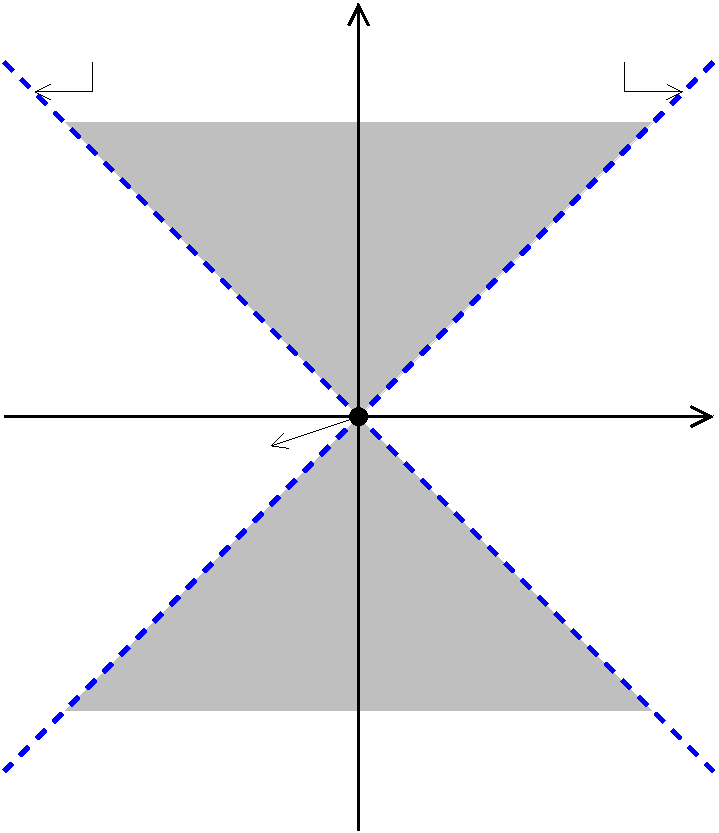
\includegraphics[scale=.5]
{src/images/lbk-graphics/light-cone2.pdf}};
\node at (0,3.75) {\small  $ct$} ;
\node at (3.15,0) [right]{\small  $x$} ;
\node at (0,1.75) {\scriptsize Absolute future 
of $P$};
\node at (0,-1.75) {\scriptsize {Absolute past of $P$}};
\node at (-0.9,-0.25){\small  $P$};
\node at (-2.25,0) [rotate=90]{\scriptsize Absolute 
elsewhere of $P$};
\node at (2.25,0) [rotate=90]{\scriptsize Absolute 
elsewhere of $P$};
\node at (-2.1,2.9) [above]{\small   $x=-ct$};
\node at (2.2,2.9) [above]{\small   $x=ct$};
\end{tikzpicture}
\end{center}
\vspace{-3mm}\caption{The light cone at an event $P$. Here, 
we have placed $P$ at the origin of the $S$-frame and have 
shown only the dimensions $x$ and $ct$.}\label{fig5.1}
\end{figure}

\index{light cone ! at an event}
Let $P:(x^\gkm_{_P})$  and $Q:(x^\gkm_{_Q})$ be any two 
events of $\mbb{M}$. Then the event $Q: (x^\gkm_\sfx{Q})$ is 
said to be separated from the event $P: (x^\gkm_\sfx{P}) $ 
by a {timelike}, {null (lightlike)} or {spacelike} interval 
according as the spacetime-interval separating  th events  
$P$ and is  $Q$ is \textsl{timelike}, \textsl{null} 
(\textsl{lightlike}) or \textsl{spacelike}:
\begin{align}\label{mw.25} 
\Delta s_\sfx{PQ}^2 \gtreqqless 0.
\end{align} 
The light cone at the event $P$ divides the 
Minkowski world $\mbb{M}$ as the union of the following 
disjoint regions\textbf{ relative to} $P$ in a Lorentz 
invariant manner:

\begin{description}

\item [The event $P$] labelled by the coordinates 
$(ct_\sfx{P},x_\sfx{P},y_\sfx{P},z_\sfx{P})$, 

\item [the absolute past of $P$] \index{lightcone ! 
absolute 
! past} which is the set of all events $Q$   satisfying  
$\Delta s_\sfx{PQ}^2 > 0,\; t_\sfx{Q}< t_\sfx{P}$, in all 
Lorentz  coordinate systems,

\item [the absolute future  of $P$] \index{lightcone ! 
absolute future} which is the set of all events $Q$ 
satisfying  $\Delta s_\sfx{PQ}^2 > 0,\; t_\sfx{Q}> 
t_\sfx{P}$, in all Lorentz frames,

\item [the forward light cone  at $P$] \index{event ! 
forward light cone of an} \index{light cone !
forward} which is the set of all events $Q$  satisfying 
$\Delta s_\sfx{PQ}^2 = 0, \quad t_\sfx{Q}>t_\sfx{P}$, in 
all Lorentz  coordinate systems, 

\item [the backward light cone at $P$] \index{event ! 
backward light cone of an} which is the set of all  events 
$Q$  satisfying $\Delta s_\sfx{PQ}^2 = 0, \quad 
t_\sfx{Q}<t_\sfx{P}$, in all  Lorentz coordinate systems, 
and 

\item [the  absolute ``elsewhere'' of $P$] \index{event ! 
absolute elsewhere of  an} which is the set of all   events 
$Q$ satisfying $ \Delta s_\sfx{PQ}^2 < 0$, in all Lorentz  
coordinate systems. 
\end{description}

Note that the above  division of $\mbb{M}$ is not a global 
partition of $\mbb{M}$ into the above mentioned regions. The 
light cone at one event $P$ is different  from the light 
cone at some other event $Q$. Moreover, it is possible that 
a given event $Q$ which is in the absolute future of the 
event $P$ may well be in the absolute past, on the light 
cone,  or in the elsewhere of some other event $P^{\,'}$.

All the events $Q$ {in the absolute future} of the event $P$ 
occur {after} $P$  and are separated from $P$ by the 
{timelike interval} $\Delta s_\sfx{PQ}^2>0$ in all Lorentz 
coordinate systems. 

Two such events $P$ and $Q$ lie on the 
timelike history of a material particle which leaves the 
spatial point corresponding to $P$  at an earlier instant of 
time and reaches the spatial point corresponding to $Q$ at a 
later instant of time (in all Lorentz coordinate systems).

All events $Q$ {in the absolute past} of the event $P$ occur 
{before} $P$ and are separated from $P$ by the {timelike 
interval} $\Delta s_\sfx{QP}^2>0$. Even here, the events $P$ 
and $Q$ lie on the timelike history of a material particle. 
A material particle which left the spatial point 
corresponding to the event $Q$ at an {earlier} instant of 
time reaches the spatial point  corresponding 
the event $P$  at a later instant of time (in all Lorentz 
coordinate systems).  All the events $Q$ {on the forward 
light cone} at $P$ 
occur {after} $P$  and are separated from $P$ by the null 
interval $\Delta s_\sfx{PQ}^2=0$ in all Lorentz coordinate 
systems. Similarly, all the events $Q$ {on the backward 
light cone} at $P$ occur {before} $P$  and are separated 
from $P$ by the {null interval} $\Delta s_\sfx{PQ}^2=0$ in 
all Lorentz coordinate systems. In both these cases, the 
event $Q$ can be connected with the event $P$ only by a 
light signal.

Lastly, every  event $Q$ {in the absolute elsewhere} of the 
event $P$ is separated from $P$ by the {spacelike 
interval}  $\Delta s_\sfx{PQ}^2<0$. The {time-ordering} 
(i.e., the relations before, simultaneous and after) of such 
an event $Q$ which is  spacelike-separated from $P$ {is not 
absolute} and can  change from one Lorentz coordinate system 
to another. Any two spacelike-events $P$ and $Q$ do not lie 
on the  history of either a material particle or of a light 
ray.

\vspace{-.2cm}

\subsection{4-tensor fields and their 
derivatives}\index{4-tensor fields ! derivatives}
\hbf{4-tensor field}If a 4-tensor of the type $(r+s)$ is 
associated with every point of a certain domain $D\in 
\mbb{M}$, possibly through some rule of association denoted 
by
\begin{align}\label{mw.26}
?A^{{\gkm_1}\dots
{\gkm_r}}_{{\gkn_1}\dots {\gkn_s}}?=?A^{{\gkm_1}\dots
{\gkm_r}}_{{\gkn_1}\dots {\gkn_s}}?(x),
\end{align}
we say that $?A^{{\gkm_1}\dots 
{\gkm_r}}_{{\gkn_1}\dots {\gkn_s}}?(x)$ is a 
\textit{4-tensor function}, or, \textit{4-tensor field}, 
defined on the domain $D\in \mbb{M}$. We must note that in 
\eqref{mw.26}, the compressed argument $(x)$ indicates a 
dependence on all the spacetime coordinates 
$(x^0,x^1,x^2,x^3)$ in general. 

\hbf{The 4-gradient operator}
Let us define a 4-component object $ \dow_\gka$ as follows:
\begin{align}\label{mw.27}
\dow_\gka =\left(\frac{1}{c}\,\frac{\dow}{\dow
t},\frac{\dow}{\dow x},\frac{\dow}{\dow 
y},\frac{\dow}{\dow z}\right) 
=\left(\frac{1}{c}\frac{\dow}{\dow t},\vnab 
\right).
\end{align}
Under a {general} coordinate transformation $x^\gka
\rightarrow {x}^{\gka'}$, we note that
\begin{align*}
\dow_{\gka'} =\frac{\dow}{\dow x^{\gka'} }=
\frac{\dow x^\gkb }{\dow x^{\gka'} }\,
\frac{\dow}{\dow x^\gkb}=
\frac{\dow x^\gkb }{\dow x'^\gka }\,\dow_\gkb,
\end{align*}
which shows that $\dow_\gka$ are the covariant components of 
a 4-vector\footnote{In fact, this transformation rule shows 
that $\dow_\gka$ are the covariant components of a vector 
(operator) under a general transformation.} operator. The 
contravariant components of this 4-gradient operator are
\begin{align}\label{mw.28}
\dow^\gka =\eta^{\gka \gkb}\dow_\gkb=
(\frac{1}{c}\frac{\dow}{\dow t},-\vnab )\,.
\end{align}

\hbf{Tensor Derivatives}\index{4-tensor fields ! 
tensor derivatives} Given a 4-tensor field of the rank 
$(r+s)$,  say, $?A^{{\gkm_1}\dots {\gkm_r}}_{{\gkn_1}\dots 
{\gkn_s}}?(x)$ all whose components are differentiable 
functions of the coordinates  defined in some domain $D\in 
\mbb{M}$, we observe that the set of all partial derivatives
\begin{align*}
(\dow/\dow 
x^\gkr)?A^{{\gkm_1}\dots {\gkm_r}}_{{\gkn_1}\dots 
{\gkn_s}}?(P)\equiv?\dow_{\gkr}??A^{{\gkm_1}\dots 
{\gkm_r}}_{{\gkn_1}\dots {\gkn_s}}?(x),                     
\end{align*}
 being the outer-product of the co-vector (operator) 
$?\dow_{\gkr}?$ and the $(r+s)$-4-tensor $?A^{{\gkm_1}\dots 
{\gkm_r}}_{{\gkn_1}\dots {\gkn_s}}?$,  is clearly a 4-tensor 
field of the type $\big(r+(s+1)\big)$ defined in $D\in 
\mbb{M}$. That is, upon partial differentiation with respect 
to $x^\gka$, the set of all partial derivatives of a 
4-tensor field (assuming the derivatives all exist) forms a 
4-tensor field whose covariant-rank has increased by $1$. 
For example, if $\phi(x)$ is a scalar field, then its 
partial derivative $\dow_\gka \phi$  is a co-4-vector field.

Raising the covariant index $\gka$ on $\dow_\gka$, we get 
the contra  -variant-4-vector operator 
$\dow^\gkb=\gky^{\gkb\gka}\dow_\gka$, using which one 
occasionally defines a 'contravariant-partial derivative'  
$\dow^\gkb T(x)$ of a tensor field  $T(x)$. Upon such an 
operation, $\dow^\gkb T(x)$ would be a tensor field whose 
contravariant rank has increased by unity over that of 
$T(x)$.

\vspace{-.3cm}

\section*{Exercises}

\vspace{-.2cm}

\exise A 4-vector $\mathbf{A}$ has vanishing contra 
components in a Lorentz coordinate system $S$. Prove that 
$\mathbf{A}$ has vanishing contra components in every other 
possible  Lorentz coordinate system $S'$ by appealing to the 
Lorentz transformation law of its components.

\exise Prove that the elements  $\gky_{\gkm\gkn}$ of the 
Minkowski matrix $\gky$ and the elements $\gky^{\gkm\gkn}$ 
of its inverse matrix $ \gky^{-1}$ are 4-tensors of the type 
$(0,2) $ and $(2,0)$.

\exise Prove that the Kronecker delta $?\delta^\gkm_\gkn?$ 
is a 4-tensor of the type $(1,1)$.

\exise We define a 4-contravector field $A^\gkm(x^\gkm) 
\equiv  A^\gkm(x)$ over a domain $D$ of $\mbb{M}$ by 
assigning a 4-contra  -vector $A^\gkm$ to each event in $D$. 
Consider a differentiable 4-contravector field $A^\gkm(x)$ 
and show that its differential $dA^\gkm$ is again a 
4-contravector field.

\exise Consider a {curve $\ell$ in $\mbb{M}$  with the 
parametric equation} $ \ell : x^\gkm=x^\gkm(\gkl), \; 
\gkl\in D_\gkl$, where $\gkl$ is an invariant (4-scalar) 
parameter on $\ell$. Prove that $T^\gkm(\gkl)\equiv 
(dx^\gkm/d\gkl)$ is a 4-contravector field defined on 
$\ell$. $T^\gkm$ is called a {tangent vector field} on 
$\ell$.

\exise A particle executes uniform motion on the unit circle 
$ x^2+y^2=1 $ in the plane $z=0$ of the Lorentz coordinate 
system $S$. With some suitable parametrisation, write down 
the (parametric) equation to the world line of the particle.
